
\section{Compressed Air Equivalent}

\emph{The compressed air equivalent system performs the same gas flows as the hydrogen part of the power generation and feed system. This system will allow analysis of the flow dynamics of the system without the use of hydrogen, allowing for a cheaper and safer system that is faster to realise. In this chapter, an overview is given of the system and the tests performed with it. The results of these tests are reviewed and compared with those of the python simulation.}

\subsection*{Testing Goals}
The main goal of the compressed air equivalent tests is to explore the flow dynamics of the system and verify that they match expected behaviour. This includes comparing results with the python simulation and verifying that using the internal volume of the CGG as a buffer is sufficient to ensure stable flow to the fuel cell during purge events.

Additionally, the compressed air tests will be used to gain experience with the fluidics hardware and explore risks like leakage before introducing hydrogen.


% Goals of compressed air equivalent tests:
% \begin{itemize}
%     \item Explore unknown risks
%     \item Verify expected system behaviour
%     \item Verify simulation results
%     \item Compare control strategies
% \end{itemize}


\subsection*{Results}
Figure~\ref{fig:air purge} show the pressure in the CGG buffer volume and the flow rate from the CGG to the fuel cell. Figure~\ref{fig:sim purge} shows the results of the python simulation during a similar time frame. The simulation also shows the pressure in the CGG buffer volume in green, which can be directly compared to the measure pressure in the air test. The simulation does not directly show the same flow rate. However, it does show the state of the fuel cell from which a flow rate can be inferred. The blue line in the simulation shows when the fuel cell is in purge mode, which corresponds to the higher flow rate in the air test. The cyan line shows when the fuel cell is in normal mode, which corresponds to the lower flow rate in the air test.

\emph{Note that the graph representing the flow rate of the air system has been scaled to improve visibility, this means that its units are no longer correct.}

During normal operation, the fuel cell consumes slightly more than the CGG produces, which causes the pressure in the buffer to decrease. When the pressure drops too low, the fuel cell is temporarily disabled to allow the buffer to fill up again. This behaviour is seen in both the simulation and the test results. The real system reacts a bit slower to the pressure changes than the simulation, which leads to slightly larger pressure fluctuations. However, the overall behaviour is very similar, which gives confidence that the simulation is accurately capturing the flow dynamics of the system.

When a purge event occurs, the fuel cell equivalent briefly consumes a lot more air, which causes a sharp drop in pressure. This too occurs both in the simulation and in the test results. In both systems the pressure drops from around 3.4 Bar to around 2 Bar. After the purge event, both systems disable the fuel cell to fill up the buffer again.

\begin{figure}
    \begin{subfigure}{\textwidth}
        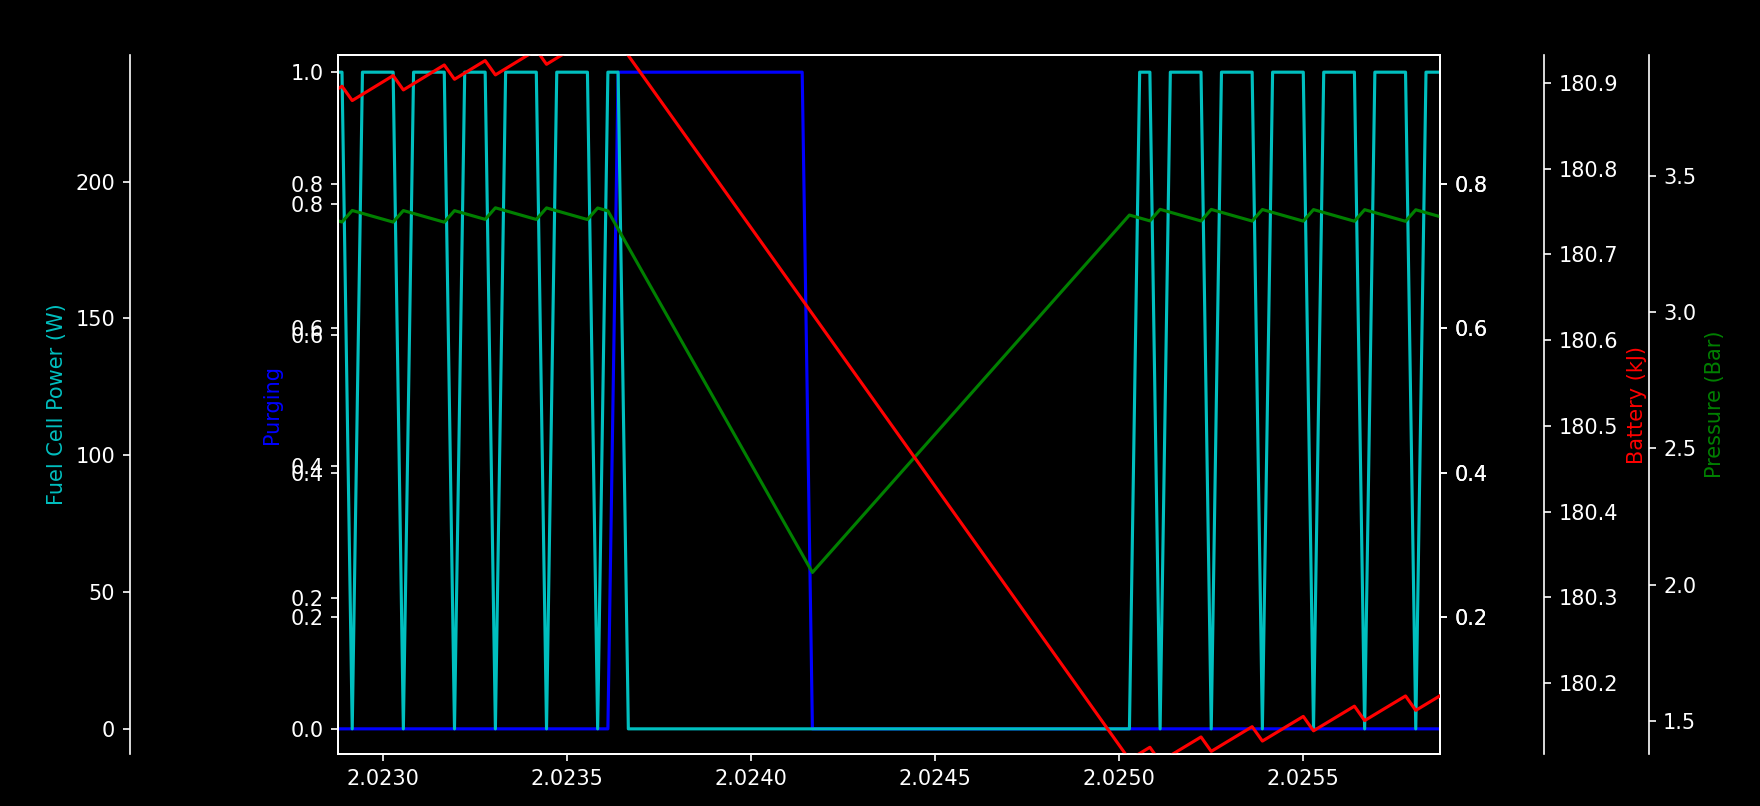
\includegraphics{media/simulated_purge.png}
        \caption{Simulated Purge Event}
        \label{fig:sim purge}
    \end{subfigure}
    \begin{subfigure}{\textwidth}
        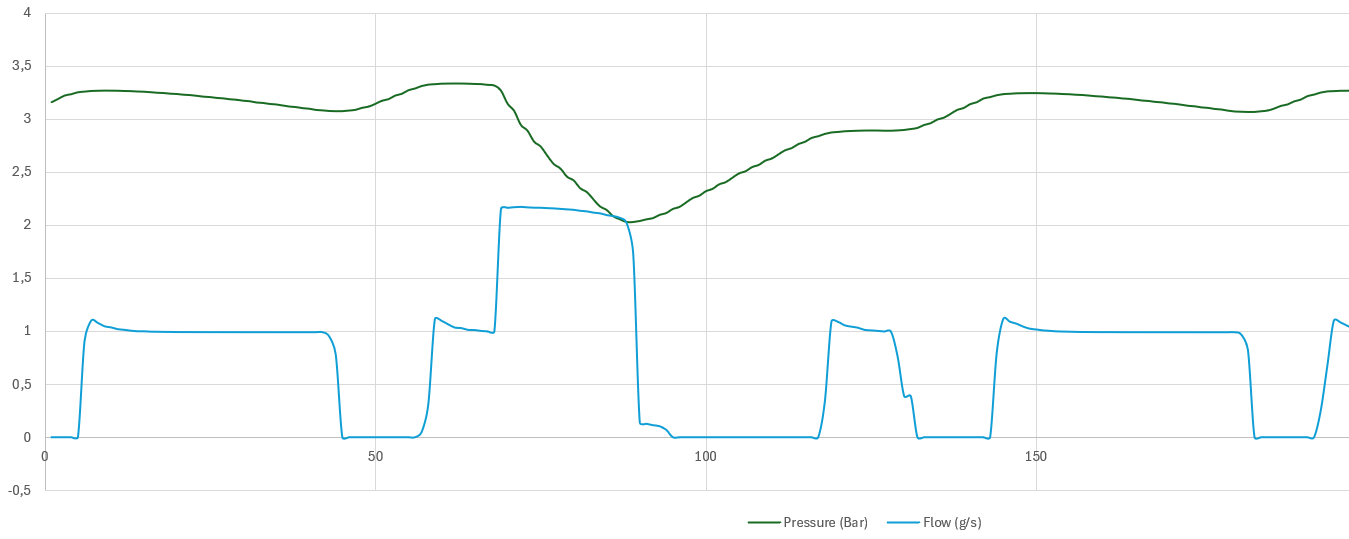
\includegraphics{media/air_purge.png}
        \caption{Measured Air Purge Event}
        \label{fig:air purge}
    \end{subfigure}
    \caption{Comparison of Simulation results with Compressed Air system}
    \label{fig:sim air comparison}
\end{figure}

\clearpage
